% filepath: /Users/__allenge/Code/Jupyter/信号与系统/Assignment15_diagram_minimal.tex
\documentclass{standalone}
\usepackage{tikz}
\usetikzlibrary{positioning, shapes, arrows}

% 定义样式(去除了填充颜色,仅保留边框)
\tikzstyle{block} = [rectangle, draw, fill=white, text centered, rounded corners, minimum height=1cm, minimum width=2cm]
\tikzstyle{sum}   = [circle, draw, fill=white, inner sep=0pt, minimum size=0.8cm]
\tikzstyle{arrow} = [->,>=stealth, line width=1pt]

\begin{document}
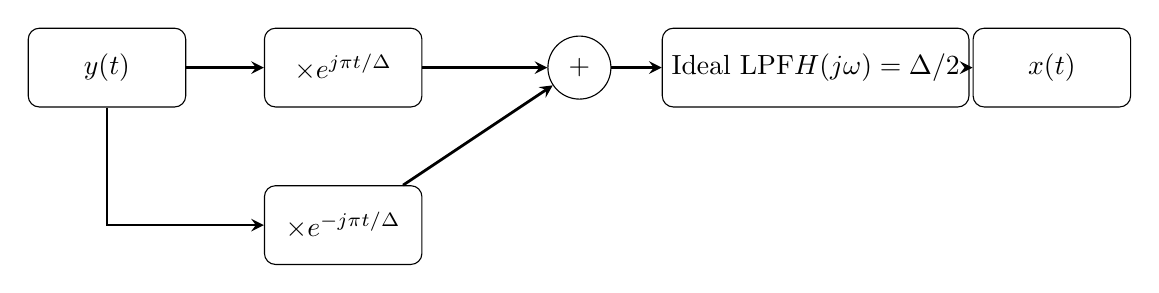
\begin{tikzpicture}[node distance=2cm, auto]
    % 输入节点
    \node [block] (y) {$y(t)$};
    
    % 第一分支:乘以 $e^{j\pi t/\Delta}$
    \node [block, right of=y, node distance=3cm] (mult1) {$\times e^{j\pi t/\Delta}$};
    
    % 第二分支:乘以 $e^{-j\pi t/\Delta}$
    \node [block, below of=mult1] (mult2) {$\times e^{-j\pi t/\Delta}$};
    
    % 叠加节点
    \node [sum, right of=mult1, node distance=3cm] (adder) {+};
    
    % 理想低通滤波器
    \node [block, right of=adder, node distance=3cm] (lpf) {Ideal LPF\\ $H(j\omega)=\Delta/2$};
    
    % 输出节点
    \node [block, right of=lpf, node distance=3cm] (x) {$x(t)$};
    
    % 画箭头
    \draw [arrow] (y) -- (mult1);
    \draw [arrow] (y) |- (mult2);
    \draw [arrow] (mult1) -- (adder);
    \draw [arrow] (mult2) -- (adder);
    \draw [arrow] (adder) -- (lpf);
    \draw [arrow] (lpf) -- (x);
\end{tikzpicture}
\end{document}